Since animals with conciousness have been around, play has been part of their lives. Cubs of predators play to prepare them for the hunt or the fight that will inevitably come. Games always have been part of the teaching of essential life skills, and humans are no different. Play comes naturally to children as breathing does, encouraging them from very early on to improve their motoric or intellectual skills, preparing them for the world ahead \cite{traditional} \cite{lifelong}.
video games in general have become an increasingly common and important form of entertainment in the US especially \cite{engage}, and have been used for over 20 years now in educational environments like schools and universities \cite{compare}.
Already in the 80s and 90s, researchers claimed that computers and computer based media could be used as an effective cognitive tool for learning and pointed out a number of other potential advantages that computer aided learning could offer \cite{aspects}.

In recent years many new approaches have been introduced and improved upon in education technology to foster skill acquisition and reinforcement, like Game-Based Learning and gamified apps and tools \cite{gamific}.
Game-Based Learning in formal education is already implemented, in some cases very successfully, particularly in environments like medicine, military, and other physical training \cite{aspects}, in which the user can get interactive training that prepares them for the tasks and problems that might arise in real life situations.
The digital games that are often used in the educational or general learning environment develop essential skills, like problem-solving, strategic thinking, resource management, planning and execution, and the adaption to change \cite{model}, and have become increasingly popular within corporate institutions and schools \cite{gamific}.

There are quite some well known examples of games that have been developed specifically for this purpose or that have been generally used in the skill aquisition setting:
\begin{itemize}
\item TopSim, by TERTIA Edusoft provides different games which are used in business education and advanced training for workers \cite{aspects}.
\item Environmental Detectives was developed by the MIT (Massachusetts Institute of Technology) and Microsoft during the Games-to-Teach project as a conceptual prototype for interactive educational entertainment \cite{aspects}.
\item The Monkey Wrench Conspiracy (1999), developed by Games2Train is a complete tutorial for a complex technical product, designed for industrial engineers to learn about new 3-D design \cite{aspects}, see Figure \ref{fig:5} \cite{monkey}.
\item The Stanley Parable (2013), developed by Galactic Cafe - originally designed to be a commercial game - is now used for educational purposes as well due to the users creative interpretations to implement the game within a learning process \cite{domestic}, see Figure \ref{fig:6} \cite{stanley}.
\item The Walking Dead (Telltale Games) and The Last of Us (Naughty Dog, 2013) have been used in classes about religion, spirituality, and ethics \cite{domestic}.
\item The Sid Meier's Civilization Franchise is commonly used to teach economics, sociology. It reached a wide enough audience for educational purposes that a new "educational update" was introduced to facilitate implementation in learning environments \cite{domestic}, see Figure \ref{fig:7} \cite{civil}.
\item In schools, games and gamification tools like Mangahigh, Abakus, and Kahoot have become more popular for the teaching of maths or languages through quizzes and drilling games, for example \cite{domestic}.
\item The classroom gamification tool ClassCraft adds a layer of an adventure game on top of the day to day school infrastructure and methodology. It turns school life and learning into a real life role-playing game (RPG) \cite{gamific} \cite{compare}.
\item Slice it! (Com2uS Studios, 2010) is an educational game that teaches Geometry on mobile devices \cite{model}.
\item E-quizzes in general are being more commonly used in situations that require repetition, gamified in a way where scores and rewards create incentives to keep playing and thus, motivate students and encourage learning \cite{gamific}.
\end{itemize}

\begin{figure}[h]
    \centering
    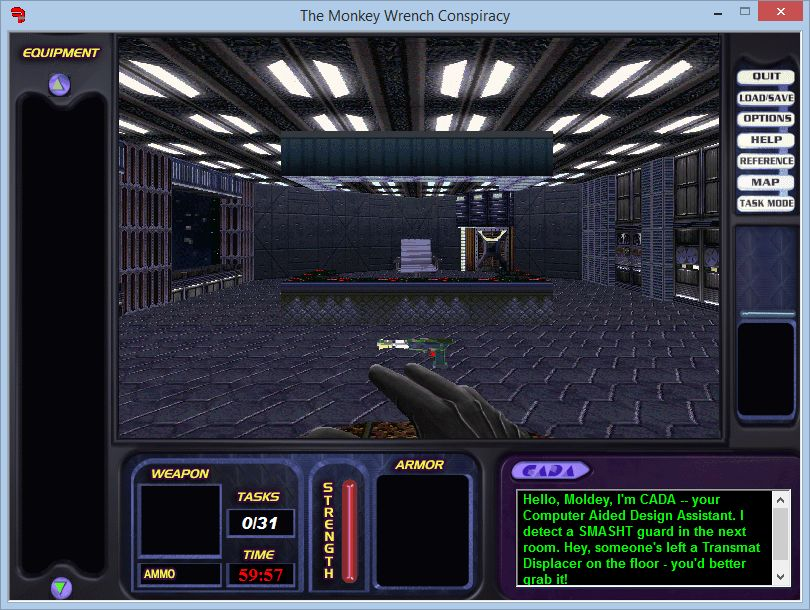
\includegraphics[width=0.6\textwidth]{figures/monkey}
    \caption{Screenshot of The Monkey Wrench Conspiracy}
    \label{fig:5}
\end{figure}

\begin{figure}[h]
    \centering
    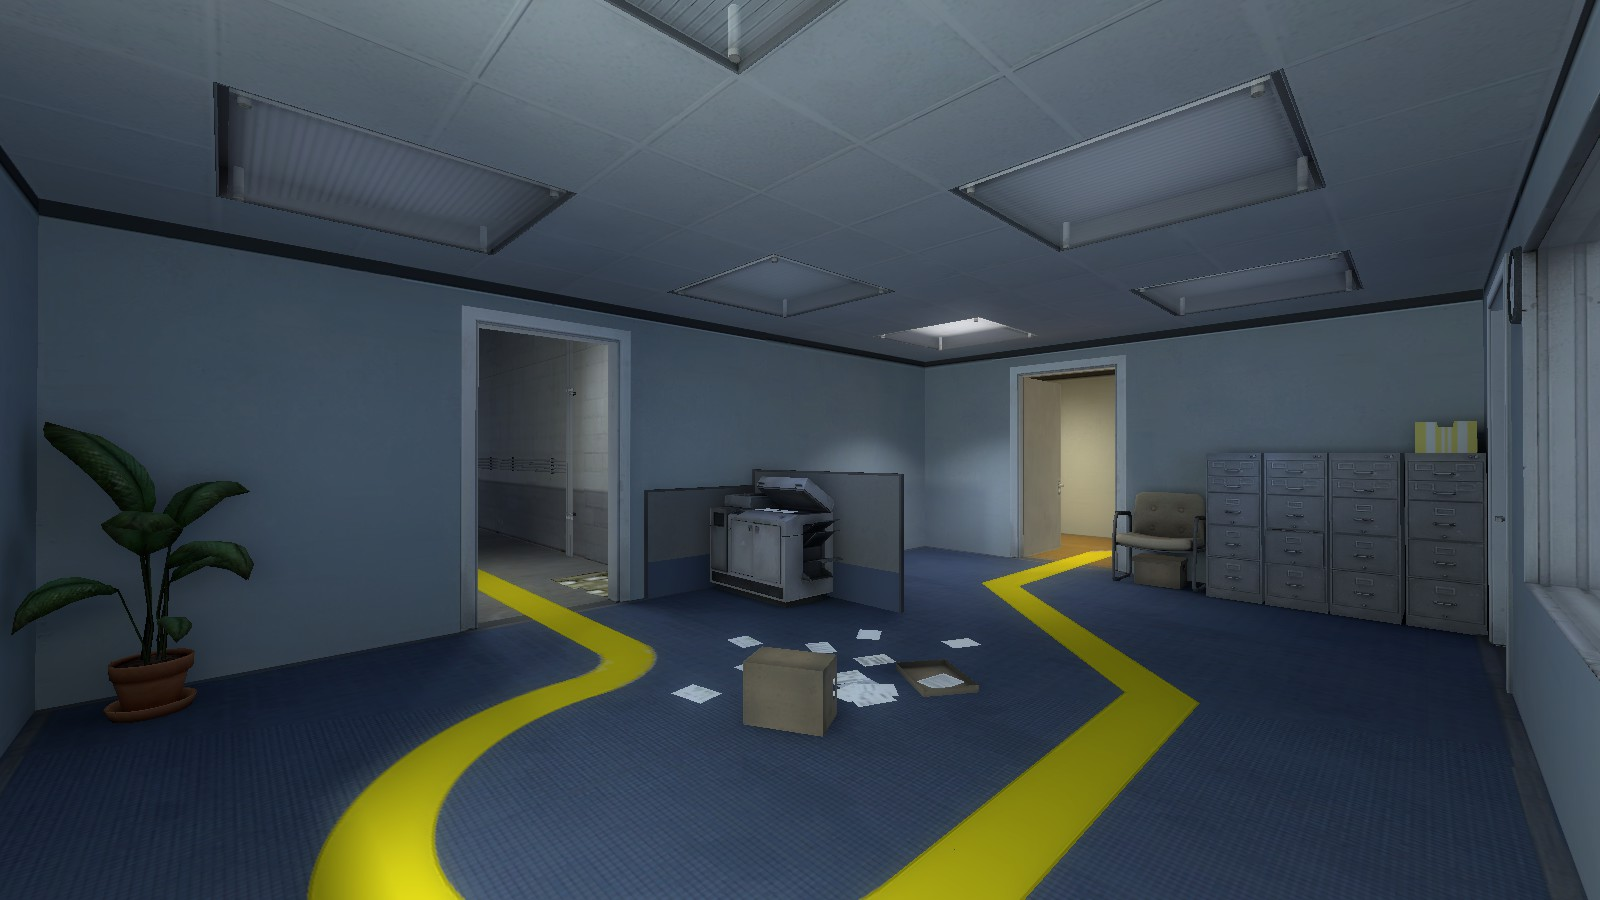
\includegraphics[width=0.6\textwidth]{figures/stanley}
    \caption{Screenshot of The Stanley Parable}
    \label{fig:6}
\end{figure}

\begin{figure}[h]
    \centering
    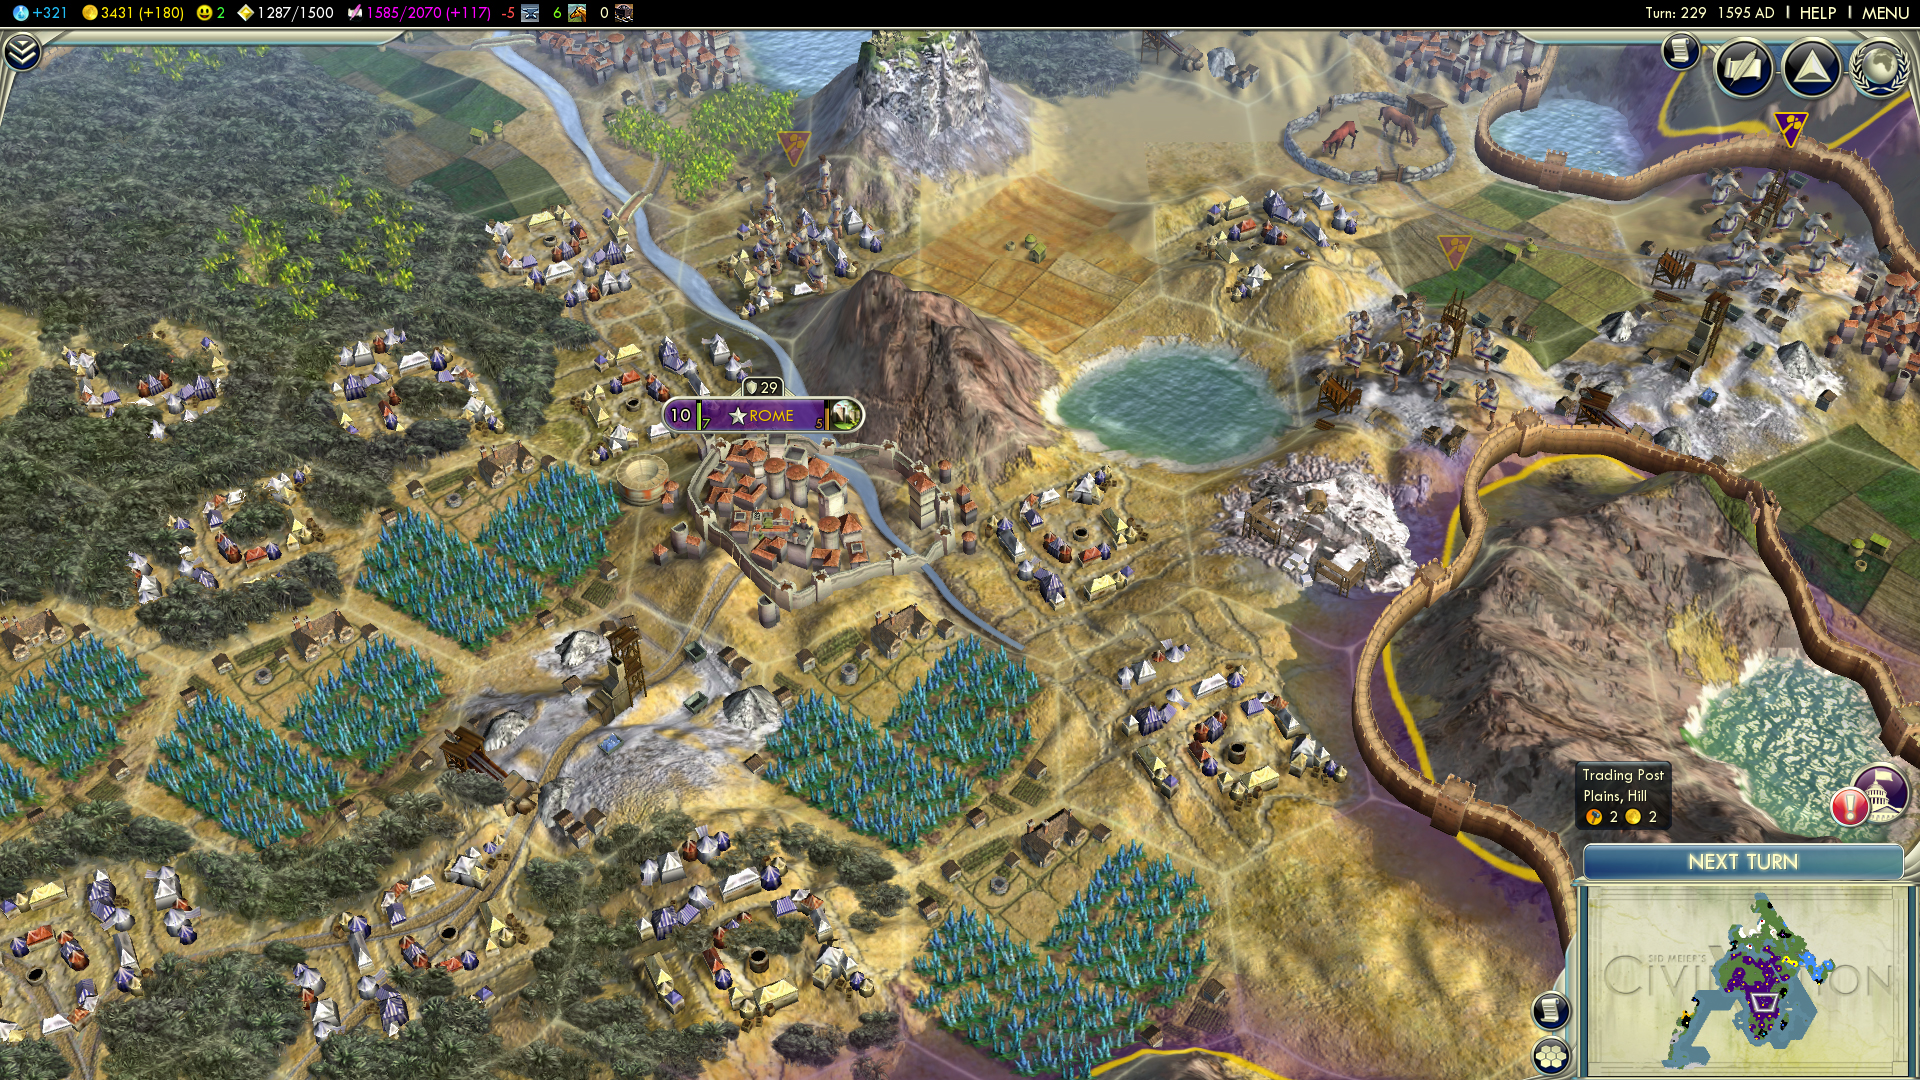
\includegraphics[width=0.6\textwidth]{figures/civil}
    \caption{Screenshot of Civilization 5}
    \label{fig:7}
\end{figure}